% Created by tikzDevice version 0.12 on 2019-01-19 16:45:02
% !TEX encoding = UTF-8 Unicode
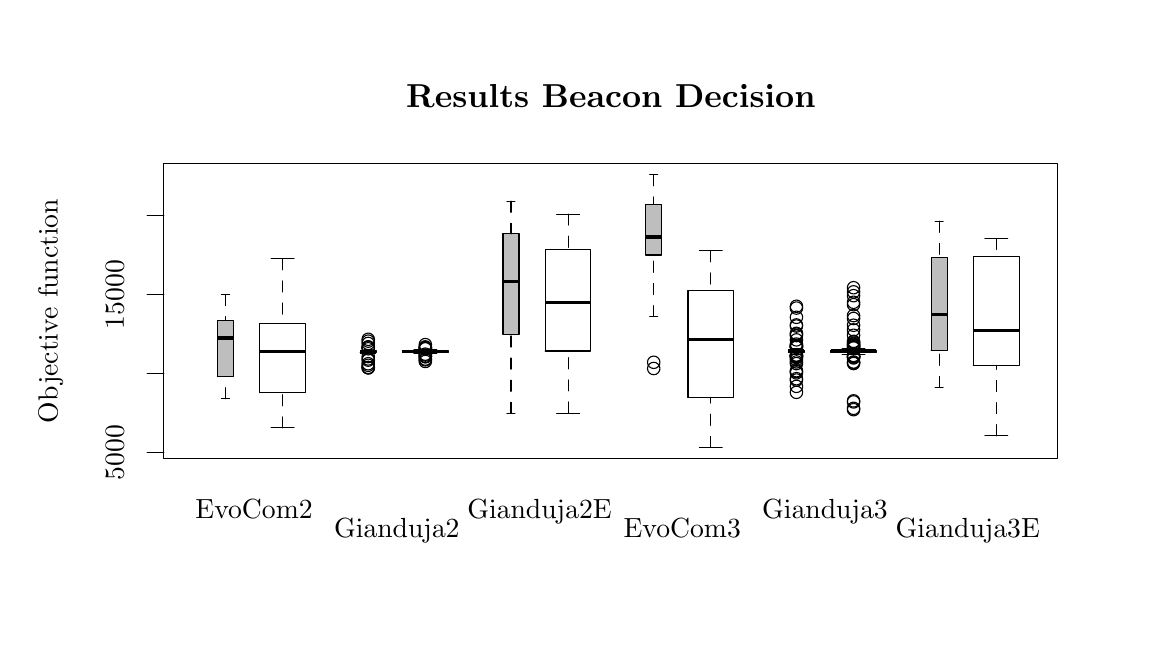
\begin{tikzpicture}[x=1pt,y=1pt]
\definecolor{fillColor}{RGB}{255,255,255}
\path[use as bounding box,fill=fillColor,fill opacity=0.00] (0,0) rectangle (397.48,216.81);
\begin{scope}
\path[clip] ( 49.20, 61.20) rectangle (372.28,167.61);
\definecolor{fillColor}{RGB}{190,190,190}

\path[fill=fillColor] ( 68.59, 90.72) --
	( 74.37, 90.72) --
	( 74.37,111.00) --
	( 68.59,111.00) --
	cycle;
\definecolor{drawColor}{RGB}{0,0,0}

\path[draw=drawColor,line width= 1.2pt,line join=round] ( 68.59,104.63) -- ( 74.37,104.63);

\path[draw=drawColor,line width= 0.4pt,dash pattern=on 4pt off 4pt ,line join=round,line cap=round] ( 71.48, 82.73) -- ( 71.48, 90.72);

\path[draw=drawColor,line width= 0.4pt,dash pattern=on 4pt off 4pt ,line join=round,line cap=round] ( 71.48,120.40) -- ( 71.48,111.00);

\path[draw=drawColor,line width= 0.4pt,line join=round,line cap=round] ( 70.04, 82.73) -- ( 72.93, 82.73);

\path[draw=drawColor,line width= 0.4pt,line join=round,line cap=round] ( 70.04,120.40) -- ( 72.93,120.40);

\path[draw=drawColor,line width= 0.4pt,line join=round,line cap=round] ( 68.59, 90.72) --
	( 74.37, 90.72) --
	( 74.37,111.00) --
	( 68.59,111.00) --
	( 68.59, 90.72);
\definecolor{fillColor}{RGB}{255,255,255}

\path[fill=fillColor] ( 83.86, 84.97) --
	(100.37, 84.97) --
	(100.37,109.94) --
	( 83.86,109.94) --
	cycle;

\path[draw=drawColor,line width= 1.2pt,line join=round] ( 83.86, 99.74) -- (100.37, 99.74);

\path[draw=drawColor,line width= 0.4pt,dash pattern=on 4pt off 4pt ,line join=round,line cap=round] ( 92.11, 72.19) -- ( 92.11, 84.97);

\path[draw=drawColor,line width= 0.4pt,dash pattern=on 4pt off 4pt ,line join=round,line cap=round] ( 92.11,133.31) -- ( 92.11,109.94);

\path[draw=drawColor,line width= 0.4pt,line join=round,line cap=round] ( 87.99, 72.19) -- ( 96.24, 72.19);

\path[draw=drawColor,line width= 0.4pt,line join=round,line cap=round] ( 87.99,133.31) -- ( 96.24,133.31);

\path[draw=drawColor,line width= 0.4pt,line join=round,line cap=round] ( 83.86, 84.97) --
	(100.37, 84.97) --
	(100.37,109.94) --
	( 83.86,109.94) --
	( 83.86, 84.97);
\definecolor{fillColor}{RGB}{190,190,190}

\path[fill=fillColor] (120.17, 99.52) --
	(125.95, 99.52) --
	(125.95, 99.98) --
	(120.17, 99.98) --
	cycle;

\path[draw=drawColor,line width= 1.2pt,line join=round] (120.17, 99.65) -- (125.95, 99.65);

\path[draw=drawColor,line width= 0.4pt,dash pattern=on 4pt off 4pt ,line join=round,line cap=round] (123.06, 99.04) -- (123.06, 99.52);

\path[draw=drawColor,line width= 0.4pt,dash pattern=on 4pt off 4pt ,line join=round,line cap=round] (123.06,100.46) -- (123.06, 99.98);

\path[draw=drawColor,line width= 0.4pt,line join=round,line cap=round] (121.62, 99.04) -- (124.50, 99.04);

\path[draw=drawColor,line width= 0.4pt,line join=round,line cap=round] (121.62,100.46) -- (124.50,100.46);

\path[draw=drawColor,line width= 0.4pt,line join=round,line cap=round] (120.17, 99.52) --
	(125.95, 99.52) --
	(125.95, 99.98) --
	(120.17, 99.98) --
	(120.17, 99.52);

\path[draw=drawColor,line width= 0.4pt,line join=round,line cap=round] (123.06,101.47) circle (  2.25);

\path[draw=drawColor,line width= 0.4pt,line join=round,line cap=round] (123.06,100.78) circle (  2.25);

\path[draw=drawColor,line width= 0.4pt,line join=round,line cap=round] (123.06, 94.81) circle (  2.25);

\path[draw=drawColor,line width= 0.4pt,line join=round,line cap=round] (123.06, 95.37) circle (  2.25);

\path[draw=drawColor,line width= 0.4pt,line join=round,line cap=round] (123.06,102.71) circle (  2.25);

\path[draw=drawColor,line width= 0.4pt,line join=round,line cap=round] (123.06, 94.04) circle (  2.25);

\path[draw=drawColor,line width= 0.4pt,line join=round,line cap=round] (123.06, 97.95) circle (  2.25);

\path[draw=drawColor,line width= 0.4pt,line join=round,line cap=round] (123.06,104.21) circle (  2.25);

\path[draw=drawColor,line width= 0.4pt,line join=round,line cap=round] (123.06, 97.11) circle (  2.25);

\path[draw=drawColor,line width= 0.4pt,line join=round,line cap=round] (123.06, 93.85) circle (  2.25);

\path[draw=drawColor,line width= 0.4pt,line join=round,line cap=round] (123.06,103.54) circle (  2.25);

\path[draw=drawColor,line width= 0.4pt,line join=round,line cap=round] (123.06, 93.97) circle (  2.25);

\path[draw=drawColor,line width= 0.4pt,line join=round,line cap=round] (123.06, 96.67) circle (  2.25);

\path[draw=drawColor,line width= 0.4pt,line join=round,line cap=round] (123.06,101.31) circle (  2.25);

\path[draw=drawColor,line width= 0.4pt,line join=round,line cap=round] (123.06,101.33) circle (  2.25);
\definecolor{fillColor}{RGB}{255,255,255}

\path[fill=fillColor] (135.44, 99.54) --
	(151.94, 99.54) --
	(151.94, 99.98) --
	(135.44, 99.98) --
	cycle;

\path[draw=drawColor,line width= 1.2pt,line join=round] (135.44, 99.88) -- (151.94, 99.88);

\path[draw=drawColor,line width= 0.4pt,dash pattern=on 4pt off 4pt ,line join=round,line cap=round] (143.69, 98.91) -- (143.69, 99.54);

\path[draw=drawColor,line width= 0.4pt,dash pattern=on 4pt off 4pt ,line join=round,line cap=round] (143.69,100.34) -- (143.69, 99.98);

\path[draw=drawColor,line width= 0.4pt,line join=round,line cap=round] (139.56, 98.91) -- (147.82, 98.91);

\path[draw=drawColor,line width= 0.4pt,line join=round,line cap=round] (139.56,100.34) -- (147.82,100.34);

\path[draw=drawColor,line width= 0.4pt,line join=round,line cap=round] (135.44, 99.54) --
	(151.94, 99.54) --
	(151.94, 99.98) --
	(135.44, 99.98) --
	(135.44, 99.54);

\path[draw=drawColor,line width= 0.4pt,line join=round,line cap=round] (143.69,100.95) circle (  2.25);

\path[draw=drawColor,line width= 0.4pt,line join=round,line cap=round] (143.69,102.28) circle (  2.25);

\path[draw=drawColor,line width= 0.4pt,line join=round,line cap=round] (143.69, 96.19) circle (  2.25);

\path[draw=drawColor,line width= 0.4pt,line join=round,line cap=round] (143.69, 98.03) circle (  2.25);

\path[draw=drawColor,line width= 0.4pt,line join=round,line cap=round] (143.69, 98.51) circle (  2.25);

\path[draw=drawColor,line width= 0.4pt,line join=round,line cap=round] (143.69,100.76) circle (  2.25);

\path[draw=drawColor,line width= 0.4pt,line join=round,line cap=round] (143.69, 97.06) circle (  2.25);

\path[draw=drawColor,line width= 0.4pt,line join=round,line cap=round] (143.69, 97.92) circle (  2.25);

\path[draw=drawColor,line width= 0.4pt,line join=round,line cap=round] (143.69,101.22) circle (  2.25);

\path[draw=drawColor,line width= 0.4pt,line join=round,line cap=round] (143.69, 96.78) circle (  2.25);

\path[draw=drawColor,line width= 0.4pt,line join=round,line cap=round] (143.69,101.45) circle (  2.25);

\path[draw=drawColor,line width= 0.4pt,line join=round,line cap=round] (143.69,101.11) circle (  2.25);

\path[draw=drawColor,line width= 0.4pt,line join=round,line cap=round] (143.69, 98.83) circle (  2.25);

\path[draw=drawColor,line width= 0.4pt,line join=round,line cap=round] (143.69, 97.95) circle (  2.25);
\definecolor{fillColor}{RGB}{190,190,190}

\path[fill=fillColor] (171.75,105.97) --
	(177.53,105.97) --
	(177.53,142.31) --
	(171.75,142.31) --
	cycle;

\path[draw=drawColor,line width= 1.2pt,line join=round] (171.75,125.13) -- (177.53,125.13);

\path[draw=drawColor,line width= 0.4pt,dash pattern=on 4pt off 4pt ,line join=round,line cap=round] (174.64, 77.42) -- (174.64,105.97);

\path[draw=drawColor,line width= 0.4pt,dash pattern=on 4pt off 4pt ,line join=round,line cap=round] (174.64,154.10) -- (174.64,142.31);

\path[draw=drawColor,line width= 0.4pt,line join=round,line cap=round] (173.19, 77.42) -- (176.08, 77.42);

\path[draw=drawColor,line width= 0.4pt,line join=round,line cap=round] (173.19,154.10) -- (176.08,154.10);

\path[draw=drawColor,line width= 0.4pt,line join=round,line cap=round] (171.75,105.97) --
	(177.53,105.97) --
	(177.53,142.31) --
	(171.75,142.31) --
	(171.75,105.97);
\definecolor{fillColor}{RGB}{255,255,255}

\path[fill=fillColor] (187.02, 99.98) --
	(203.52, 99.98) --
	(203.52,136.70) --
	(187.02,136.70) --
	cycle;

\path[draw=drawColor,line width= 1.2pt,line join=round] (187.02,117.59) -- (203.52,117.59);

\path[draw=drawColor,line width= 0.4pt,dash pattern=on 4pt off 4pt ,line join=round,line cap=round] (195.27, 77.54) -- (195.27, 99.98);

\path[draw=drawColor,line width= 0.4pt,dash pattern=on 4pt off 4pt ,line join=round,line cap=round] (195.27,149.45) -- (195.27,136.70);

\path[draw=drawColor,line width= 0.4pt,line join=round,line cap=round] (191.14, 77.54) -- (199.40, 77.54);

\path[draw=drawColor,line width= 0.4pt,line join=round,line cap=round] (191.14,149.45) -- (199.40,149.45);

\path[draw=drawColor,line width= 0.4pt,line join=round,line cap=round] (187.02, 99.98) --
	(203.52, 99.98) --
	(203.52,136.70) --
	(187.02,136.70) --
	(187.02, 99.98);
\definecolor{fillColor}{RGB}{190,190,190}

\path[fill=fillColor] (223.33,134.67) --
	(229.10,134.67) --
	(229.10,152.99) --
	(223.33,152.99) --
	cycle;

\path[draw=drawColor,line width= 1.2pt,line join=round] (223.33,141.22) -- (229.10,141.22);

\path[draw=drawColor,line width= 0.4pt,dash pattern=on 4pt off 4pt ,line join=round,line cap=round] (226.22,112.40) -- (226.22,134.67);

\path[draw=drawColor,line width= 0.4pt,dash pattern=on 4pt off 4pt ,line join=round,line cap=round] (226.22,163.67) -- (226.22,152.99);

\path[draw=drawColor,line width= 0.4pt,line join=round,line cap=round] (224.77,112.40) -- (227.66,112.40);

\path[draw=drawColor,line width= 0.4pt,line join=round,line cap=round] (224.77,163.67) -- (227.66,163.67);

\path[draw=drawColor,line width= 0.4pt,line join=round,line cap=round] (223.33,134.67) --
	(229.10,134.67) --
	(229.10,152.99) --
	(223.33,152.99) --
	(223.33,134.67);

\path[draw=drawColor,line width= 0.4pt,line join=round,line cap=round] (226.22, 95.90) circle (  2.25);

\path[draw=drawColor,line width= 0.4pt,line join=round,line cap=round] (226.22, 93.65) circle (  2.25);
\definecolor{fillColor}{RGB}{255,255,255}

\path[fill=fillColor] (238.59, 83.18) --
	(255.10, 83.18) --
	(255.10,121.82) --
	(238.59,121.82) --
	cycle;

\path[draw=drawColor,line width= 1.2pt,line join=round] (238.59,104.11) -- (255.10,104.11);

\path[draw=drawColor,line width= 0.4pt,dash pattern=on 4pt off 4pt ,line join=round,line cap=round] (246.85, 65.14) -- (246.85, 83.18);

\path[draw=drawColor,line width= 0.4pt,dash pattern=on 4pt off 4pt ,line join=round,line cap=round] (246.85,136.19) -- (246.85,121.82);

\path[draw=drawColor,line width= 0.4pt,line join=round,line cap=round] (242.72, 65.14) -- (250.97, 65.14);

\path[draw=drawColor,line width= 0.4pt,line join=round,line cap=round] (242.72,136.19) -- (250.97,136.19);

\path[draw=drawColor,line width= 0.4pt,line join=round,line cap=round] (238.59, 83.18) --
	(255.10, 83.18) --
	(255.10,121.82) --
	(238.59,121.82) --
	(238.59, 83.18);
\definecolor{fillColor}{RGB}{190,190,190}

\path[fill=fillColor] (274.91, 99.54) --
	(280.68, 99.54) --
	(280.68,100.18) --
	(274.91,100.18) --
	cycle;

\path[draw=drawColor,line width= 1.2pt,line join=round] (274.91, 99.96) -- (280.68, 99.96);

\path[draw=drawColor,line width= 0.4pt,dash pattern=on 4pt off 4pt ,line join=round,line cap=round] (277.79, 98.63) -- (277.79, 99.54);

\path[draw=drawColor,line width= 0.4pt,dash pattern=on 4pt off 4pt ,line join=round,line cap=round] (277.79,100.91) -- (277.79,100.18);

\path[draw=drawColor,line width= 0.4pt,line join=round,line cap=round] (276.35, 98.63) -- (279.24, 98.63);

\path[draw=drawColor,line width= 0.4pt,line join=round,line cap=round] (276.35,100.91) -- (279.24,100.91);

\path[draw=drawColor,line width= 0.4pt,line join=round,line cap=round] (274.91, 99.54) --
	(280.68, 99.54) --
	(280.68,100.18) --
	(274.91,100.18) --
	(274.91, 99.54);

\path[draw=drawColor,line width= 0.4pt,line join=round,line cap=round] (277.79,101.76) circle (  2.25);

\path[draw=drawColor,line width= 0.4pt,line join=round,line cap=round] (277.79,101.68) circle (  2.25);

\path[draw=drawColor,line width= 0.4pt,line join=round,line cap=round] (277.79,101.75) circle (  2.25);

\path[draw=drawColor,line width= 0.4pt,line join=round,line cap=round] (277.79,116.14) circle (  2.25);

\path[draw=drawColor,line width= 0.4pt,line join=round,line cap=round] (277.79, 92.86) circle (  2.25);

\path[draw=drawColor,line width= 0.4pt,line join=round,line cap=round] (277.79, 97.86) circle (  2.25);

\path[draw=drawColor,line width= 0.4pt,line join=round,line cap=round] (277.79, 98.53) circle (  2.25);

\path[draw=drawColor,line width= 0.4pt,line join=round,line cap=round] (277.79,106.36) circle (  2.25);

\path[draw=drawColor,line width= 0.4pt,line join=round,line cap=round] (277.79, 96.88) circle (  2.25);

\path[draw=drawColor,line width= 0.4pt,line join=round,line cap=round] (277.79,103.99) circle (  2.25);

\path[draw=drawColor,line width= 0.4pt,line join=round,line cap=round] (277.79, 92.05) circle (  2.25);

\path[draw=drawColor,line width= 0.4pt,line join=round,line cap=round] (277.79, 95.42) circle (  2.25);

\path[draw=drawColor,line width= 0.4pt,line join=round,line cap=round] (277.79,101.40) circle (  2.25);

\path[draw=drawColor,line width= 0.4pt,line join=round,line cap=round] (277.79,101.97) circle (  2.25);

\path[draw=drawColor,line width= 0.4pt,line join=round,line cap=round] (277.79, 97.62) circle (  2.25);

\path[draw=drawColor,line width= 0.4pt,line join=round,line cap=round] (277.79, 96.01) circle (  2.25);

\path[draw=drawColor,line width= 0.4pt,line join=round,line cap=round] (277.79,101.32) circle (  2.25);

\path[draw=drawColor,line width= 0.4pt,line join=round,line cap=round] (277.79, 87.20) circle (  2.25);

\path[draw=drawColor,line width= 0.4pt,line join=round,line cap=round] (277.79,105.54) circle (  2.25);

\path[draw=drawColor,line width= 0.4pt,line join=round,line cap=round] (277.79, 85.04) circle (  2.25);

\path[draw=drawColor,line width= 0.4pt,line join=round,line cap=round] (277.79,112.15) circle (  2.25);

\path[draw=drawColor,line width= 0.4pt,line join=round,line cap=round] (277.79, 89.96) circle (  2.25);

\path[draw=drawColor,line width= 0.4pt,line join=round,line cap=round] (277.79,106.05) circle (  2.25);

\path[draw=drawColor,line width= 0.4pt,line join=round,line cap=round] (277.79,115.50) circle (  2.25);

\path[draw=drawColor,line width= 0.4pt,line join=round,line cap=round] (277.79, 98.02) circle (  2.25);

\path[draw=drawColor,line width= 0.4pt,line join=round,line cap=round] (277.79, 98.32) circle (  2.25);

\path[draw=drawColor,line width= 0.4pt,line join=round,line cap=round] (277.79,109.00) circle (  2.25);

\path[draw=drawColor,line width= 0.4pt,line join=round,line cap=round] (277.79, 89.48) circle (  2.25);

\path[draw=drawColor,line width= 0.4pt,line join=round,line cap=round] (277.79,109.39) circle (  2.25);

\path[draw=drawColor,line width= 0.4pt,line join=round,line cap=round] (277.79, 92.53) circle (  2.25);

\path[draw=drawColor,line width= 0.4pt,line join=round,line cap=round] (277.79, 98.33) circle (  2.25);

\path[draw=drawColor,line width= 0.4pt,line join=round,line cap=round] (277.79,102.47) circle (  2.25);

\path[draw=drawColor,line width= 0.4pt,line join=round,line cap=round] (277.79, 98.20) circle (  2.25);
\definecolor{fillColor}{RGB}{255,255,255}

\path[fill=fillColor] (290.17, 99.54) --
	(306.68, 99.54) --
	(306.68,100.12) --
	(290.17,100.12) --
	cycle;

\path[draw=drawColor,line width= 1.2pt,line join=round] (290.17, 99.98) -- (306.68, 99.98);

\path[draw=drawColor,line width= 0.4pt,dash pattern=on 4pt off 4pt ,line join=round,line cap=round] (298.43, 98.76) -- (298.43, 99.54);

\path[draw=drawColor,line width= 0.4pt,dash pattern=on 4pt off 4pt ,line join=round,line cap=round] (298.43,100.69) -- (298.43,100.12);

\path[draw=drawColor,line width= 0.4pt,line join=round,line cap=round] (294.30, 98.76) -- (302.55, 98.76);

\path[draw=drawColor,line width= 0.4pt,line join=round,line cap=round] (294.30,100.69) -- (302.55,100.69);

\path[draw=drawColor,line width= 0.4pt,line join=round,line cap=round] (290.17, 99.54) --
	(306.68, 99.54) --
	(306.68,100.12) --
	(290.17,100.12) --
	(290.17, 99.54);

\path[draw=drawColor,line width= 0.4pt,line join=round,line cap=round] (298.43,103.47) circle (  2.25);

\path[draw=drawColor,line width= 0.4pt,line join=round,line cap=round] (298.43,122.84) circle (  2.25);

\path[draw=drawColor,line width= 0.4pt,line join=round,line cap=round] (298.43,101.16) circle (  2.25);

\path[draw=drawColor,line width= 0.4pt,line join=round,line cap=round] (298.43, 97.96) circle (  2.25);

\path[draw=drawColor,line width= 0.4pt,line join=round,line cap=round] (298.43,105.65) circle (  2.25);

\path[draw=drawColor,line width= 0.4pt,line join=round,line cap=round] (298.43, 97.47) circle (  2.25);

\path[draw=drawColor,line width= 0.4pt,line join=round,line cap=round] (298.43, 96.00) circle (  2.25);

\path[draw=drawColor,line width= 0.4pt,line join=round,line cap=round] (298.43, 97.90) circle (  2.25);

\path[draw=drawColor,line width= 0.4pt,line join=round,line cap=round] (298.43,102.39) circle (  2.25);

\path[draw=drawColor,line width= 0.4pt,line join=round,line cap=round] (298.43,102.74) circle (  2.25);

\path[draw=drawColor,line width= 0.4pt,line join=round,line cap=round] (298.43,103.22) circle (  2.25);

\path[draw=drawColor,line width= 0.4pt,line join=round,line cap=round] (298.43, 95.75) circle (  2.25);

\path[draw=drawColor,line width= 0.4pt,line join=round,line cap=round] (298.43,107.61) circle (  2.25);

\path[draw=drawColor,line width= 0.4pt,line join=round,line cap=round] (298.43, 79.26) circle (  2.25);

\path[draw=drawColor,line width= 0.4pt,line join=round,line cap=round] (298.43,112.76) circle (  2.25);

\path[draw=drawColor,line width= 0.4pt,line join=round,line cap=round] (298.43, 81.58) circle (  2.25);

\path[draw=drawColor,line width= 0.4pt,line join=round,line cap=round] (298.43,117.58) circle (  2.25);

\path[draw=drawColor,line width= 0.4pt,line join=round,line cap=round] (298.43,109.28) circle (  2.25);

\path[draw=drawColor,line width= 0.4pt,line join=round,line cap=round] (298.43, 78.78) circle (  2.25);

\path[draw=drawColor,line width= 0.4pt,line join=round,line cap=round] (298.43,119.97) circle (  2.25);

\path[draw=drawColor,line width= 0.4pt,line join=round,line cap=round] (298.43,116.72) circle (  2.25);

\path[draw=drawColor,line width= 0.4pt,line join=round,line cap=round] (298.43, 95.44) circle (  2.25);

\path[draw=drawColor,line width= 0.4pt,line join=round,line cap=round] (298.43,101.96) circle (  2.25);

\path[draw=drawColor,line width= 0.4pt,line join=round,line cap=round] (298.43,102.05) circle (  2.25);

\path[draw=drawColor,line width= 0.4pt,line join=round,line cap=round] (298.43,101.52) circle (  2.25);

\path[draw=drawColor,line width= 0.4pt,line join=round,line cap=round] (298.43, 98.38) circle (  2.25);

\path[draw=drawColor,line width= 0.4pt,line join=round,line cap=round] (298.43, 81.96) circle (  2.25);

\path[draw=drawColor,line width= 0.4pt,line join=round,line cap=round] (298.43,121.34) circle (  2.25);

\path[draw=drawColor,line width= 0.4pt,line join=round,line cap=round] (298.43, 97.90) circle (  2.25);

\path[draw=drawColor,line width= 0.4pt,line join=round,line cap=round] (298.43, 97.77) circle (  2.25);

\path[draw=drawColor,line width= 0.4pt,line join=round,line cap=round] (298.43,111.72) circle (  2.25);

\path[draw=drawColor,line width= 0.4pt,line join=round,line cap=round] (298.43,101.09) circle (  2.25);
\definecolor{fillColor}{RGB}{190,190,190}

\path[fill=fillColor] (326.48,100.16) --
	(332.26,100.16) --
	(332.26,133.92) --
	(326.48,133.92) --
	cycle;

\path[draw=drawColor,line width= 1.2pt,line join=round] (326.48,113.08) -- (332.26,113.08);

\path[draw=drawColor,line width= 0.4pt,dash pattern=on 4pt off 4pt ,line join=round,line cap=round] (329.37, 86.82) -- (329.37,100.16);

\path[draw=drawColor,line width= 0.4pt,dash pattern=on 4pt off 4pt ,line join=round,line cap=round] (329.37,146.87) -- (329.37,133.92);

\path[draw=drawColor,line width= 0.4pt,line join=round,line cap=round] (327.93, 86.82) -- (330.82, 86.82);

\path[draw=drawColor,line width= 0.4pt,line join=round,line cap=round] (327.93,146.87) -- (330.82,146.87);

\path[draw=drawColor,line width= 0.4pt,line join=round,line cap=round] (326.48,100.16) --
	(332.26,100.16) --
	(332.26,133.92) --
	(326.48,133.92) --
	(326.48,100.16);
\definecolor{fillColor}{RGB}{255,255,255}

\path[fill=fillColor] (341.75, 94.72) --
	(358.26, 94.72) --
	(358.26,134.14) --
	(341.75,134.14) --
	cycle;

\path[draw=drawColor,line width= 1.2pt,line join=round] (341.75,107.27) -- (358.26,107.27);

\path[draw=drawColor,line width= 0.4pt,dash pattern=on 4pt off 4pt ,line join=round,line cap=round] (350.00, 69.33) -- (350.00, 94.72);

\path[draw=drawColor,line width= 0.4pt,dash pattern=on 4pt off 4pt ,line join=round,line cap=round] (350.00,140.66) -- (350.00,134.14);

\path[draw=drawColor,line width= 0.4pt,line join=round,line cap=round] (345.88, 69.33) -- (354.13, 69.33);

\path[draw=drawColor,line width= 0.4pt,line join=round,line cap=round] (345.88,140.66) -- (354.13,140.66);

\path[draw=drawColor,line width= 0.4pt,line join=round,line cap=round] (341.75, 94.72) --
	(358.26, 94.72) --
	(358.26,134.14) --
	(341.75,134.14) --
	(341.75, 94.72);
\end{scope}
\begin{scope}
\path[clip] (  0.00,  0.00) rectangle (397.48,216.81);
\definecolor{drawColor}{RGB}{0,0,0}

\node[text=drawColor,rotate= 90.00,anchor=base,inner sep=0pt, outer sep=0pt, scale=  1.00] at ( 10.80,114.41) {Objective function};
\end{scope}
\begin{scope}
\path[clip] (  0.00,  0.00) rectangle (397.48,216.81);
\definecolor{drawColor}{RGB}{0,0,0}

\node[text=drawColor,anchor=base,inner sep=0pt, outer sep=0pt, scale=  1.00] at ( 81.80, 39.60) {EvoCom2};

\node[text=drawColor,anchor=base,inner sep=0pt, outer sep=0pt, scale=  1.00] at (184.95, 39.60) {Gianduja2E};

\node[text=drawColor,anchor=base,inner sep=0pt, outer sep=0pt, scale=  1.00] at (288.11, 39.60) {Gianduja3};

\node[text=drawColor,anchor=base,inner sep=0pt, outer sep=0pt, scale=  1.00] at (133.38, 32.71) {Gianduja2};

\node[text=drawColor,anchor=base,inner sep=0pt, outer sep=0pt, scale=  1.00] at (236.53, 32.71) {EvoCom3};

\node[text=drawColor,anchor=base,inner sep=0pt, outer sep=0pt, scale=  1.00] at (339.69, 32.71) {Gianduja3E};
\end{scope}
\begin{scope}
\path[clip] (  0.00,  0.00) rectangle (397.48,216.81);
\definecolor{drawColor}{RGB}{0,0,0}

\node[text=drawColor,anchor=base,inner sep=0pt, outer sep=0pt, scale=  1.20] at (210.74,188.07) {\bfseries Results Beacon Decision};
\end{scope}
\begin{scope}
\path[clip] (  0.00,  0.00) rectangle (397.48,216.81);
\definecolor{drawColor}{RGB}{0,0,0}

\path[draw=drawColor,line width= 0.4pt,line join=round,line cap=round] ( 49.20, 63.19) -- ( 49.20,148.89);

\path[draw=drawColor,line width= 0.4pt,line join=round,line cap=round] ( 49.20, 63.19) -- ( 43.20, 63.19);

\path[draw=drawColor,line width= 0.4pt,line join=round,line cap=round] ( 49.20, 91.76) -- ( 43.20, 91.76);

\path[draw=drawColor,line width= 0.4pt,line join=round,line cap=round] ( 49.20,120.33) -- ( 43.20,120.33);

\path[draw=drawColor,line width= 0.4pt,line join=round,line cap=round] ( 49.20,148.89) -- ( 43.20,148.89);

\node[text=drawColor,rotate= 90.00,anchor=base,inner sep=0pt, outer sep=0pt, scale=  1.00] at ( 34.80, 63.19) {5000};

\node[text=drawColor,rotate= 90.00,anchor=base,inner sep=0pt, outer sep=0pt, scale=  1.00] at ( 34.80,120.33) {15000};

\path[draw=drawColor,line width= 0.4pt,line join=round,line cap=round] ( 49.20, 61.20) --
	(372.28, 61.20) --
	(372.28,167.61) --
	( 49.20,167.61) --
	( 49.20, 61.20);
\end{scope}
\end{tikzpicture}
